% \documentclass[t, 10pt]{beamer}
\documentclass[t,handout, 10pt]{beamer}

\usepackage{graphicx}
\usepackage{epsfig}
\usepackage{psfrag}
\usepackage[english]{babel}
\usepackage{color}
\usepackage{amsmath}
\usepackage{mathrsfs}
\usepackage{amsfonts}
\usepackage{booktabs}
\usepackage{xcolor}
\usepackage{textcomp}
\usepackage{listings}
\usepackage{courier}
\usepackage{framed}
\usepackage{enumerate}
\usepackage{microtype}
\usepackage{multirow}

\lstset{
	language=Ruby,
	basicstyle=\scriptsize\ttfamily, 
	numbers=left,    
	numberstyle=\tiny,
	stepnumber=1,
	numbersep=5pt,
	tabsize=2,
	extendedchars=true,        
	breaklines=true,            
	keywordstyle=\color{red},
	frame=b,         
	stringstyle=\color{white}\ttfamily,
	showspaces=false,
	showtabs=false,
	xleftmargin=17pt,
	framexleftmargin=17pt,
	framexrightmargin=5pt,
	framexbottommargin=4pt,
	showstringspaces=false      
}

\usepackage{caption}
\DeclareCaptionFont{white}{\color{white}}
\DeclareCaptionFormat{listing}{\colorbox[cmyk]{0.43, 0.35, 0.35,0.01}{\parbox{\textwidth}{\hspace{15pt}#1#2#3}}}
\captionsetup[lstlisting]{format=listing,labelfont=white,textfont=white, singlelinecheck=false, margin=0pt, font={bf,footnotesize}}

\graphicspath{{./images/}} % Figures path - used in graphicx

\selectcolormodel{cmyk}

\mode<presentation>

%THEMES - Please refer to these chapters in the beamer documentation.
% Presentation themes : Chapter 15
% Color themes : Chapter 17
% Font themes : Chapter 18

\usetheme{Pittsburgh}
\usecolortheme{orchid}
\usefonttheme{default}

%---------------------------Title frame definition------------------------------------- 

\title{Usage Management In Multi-level Security Environments}
\author [Greg, Chris]{Gregory Heileman and Christopher C. Lamb}
\institute[University of New Mexico]{
\inst {}Department of Electrical and Computer Engineering\\
University of New Mexico}
\date{April 4, 2012}
\titlegraphic{
\begin{figure} 

\includegraphics[width = 10cm]{ECE-UNM-logo}
\end{figure}}

\begin{document}

\begin{frame}
\titlepage
\end{frame}

% This command will make the logo appear on all frames excluding the title frame.
\logo {
\includegraphics[width = 2.5cm]{UNM}}

\begin{frame}
\frametitle{Introduction}
\tableofcontents 
\end{frame}

\section{Information-centric Networking}
\begin{frame}
\frametitle{Information-centric Networking}

Information-centric networking (ICN) is a new approach to internet-scale networks.  These networks take advantage of data locality, cache data aggressively, decouple information providers from consumers, and use a content-centric perspective in network design
\pause
\newline
\newline
Similar conceptual approaches:
{\small
\begin{itemize}
\item {\bf Named Data Objects} --- Data objects are the primary data abstraction.
\item {\bf API Structure} --- Programming interfaces are structured around requesting specific data objects.  Can be synchronous or asynchronous.
\item {\bf Naming and Security} --- Names are tightly and securely bound to content.
\item {\bf Caching} --- Content is aggressively cached on nodes.
\end{itemize}
}
\pause
We are most concerned with the first and second characteristics currently.
\end{frame}

\begin{frame}
\frametitle{Current Technology Fail}
Current internet technologies don't dynamically protect data.  Initial design assumtions and implementation characteristics make these approaches difficult.
\pause
\newline
\newline
Why does the internet fail?
{\small
\begin{itemize}
\item {\bf Strict Layering} --- Routing and switching are generally lower level operations (layers 2 and 3 in the OSI model).  Content-sensitive routing is a layer 7 (application layer) operation, requiring very expensive hardware to do well. 
\item {\bf End-to-End Arguments} --- Network cores are simple, fast, and dumb.  They need to brighten up to evanluate information suitability.  
\item {\bf Packetization} --- Policies and content requires multiple packets.  This implies complex window retention logic to handle context splitting, and in at least half of typical cases, context splitting can't be handled at all.
\end{itemize}
}
The principles have been effective, but in some cases services {\it should} be in the network core.
\end{frame}

\section{System Overview}
\begin{frame}
\frametitle{System Overview --- Device Perspective}
\centerline{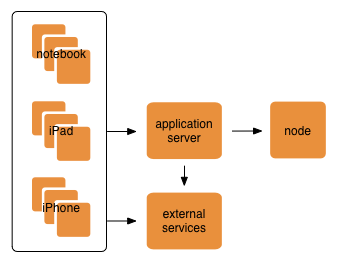
\includegraphics[width=2in]{overall-view}}
How does the system work?
\pause
{\small
\begin{enumerate}
\item {\bf Request} --- An initial request is submitted from an edge device
\pause
\item {\bf Reciept} --- The request is received by an application server that has access to ICN services via an ICN node and external services of some kind as well.
\pause
\item {\bf Dispatch} --- The request for information if suitable is dispatched into the ICN.
\end{enumerate}
}
\end{frame}

\begin{frame}
\frametitle{System Overview --- Into the network}
\centerline{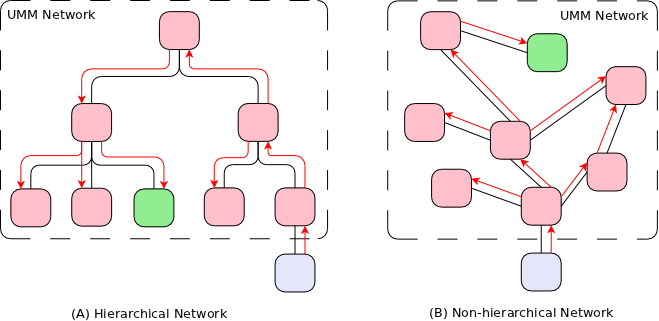
\includegraphics[width=3.5in]{node-hierarchy}}
How is information dispatched through the network? {\it Well, it depends on the network.}
\pause
{\small
\begin{enumerate}
\item {\bf Submission} --- Submit to a node.
\item {\bf Transmission} --- Pass through the network, either via a router (if hierarchical) or known peers (non-hierarchical).
\item {\bf Respond} --- Nodes respond with content if possible.
\end{enumerate}
}
\end{frame}

\begin{frame}
\frametitle{System Overivew --- Nodes and Routers}
\centerline{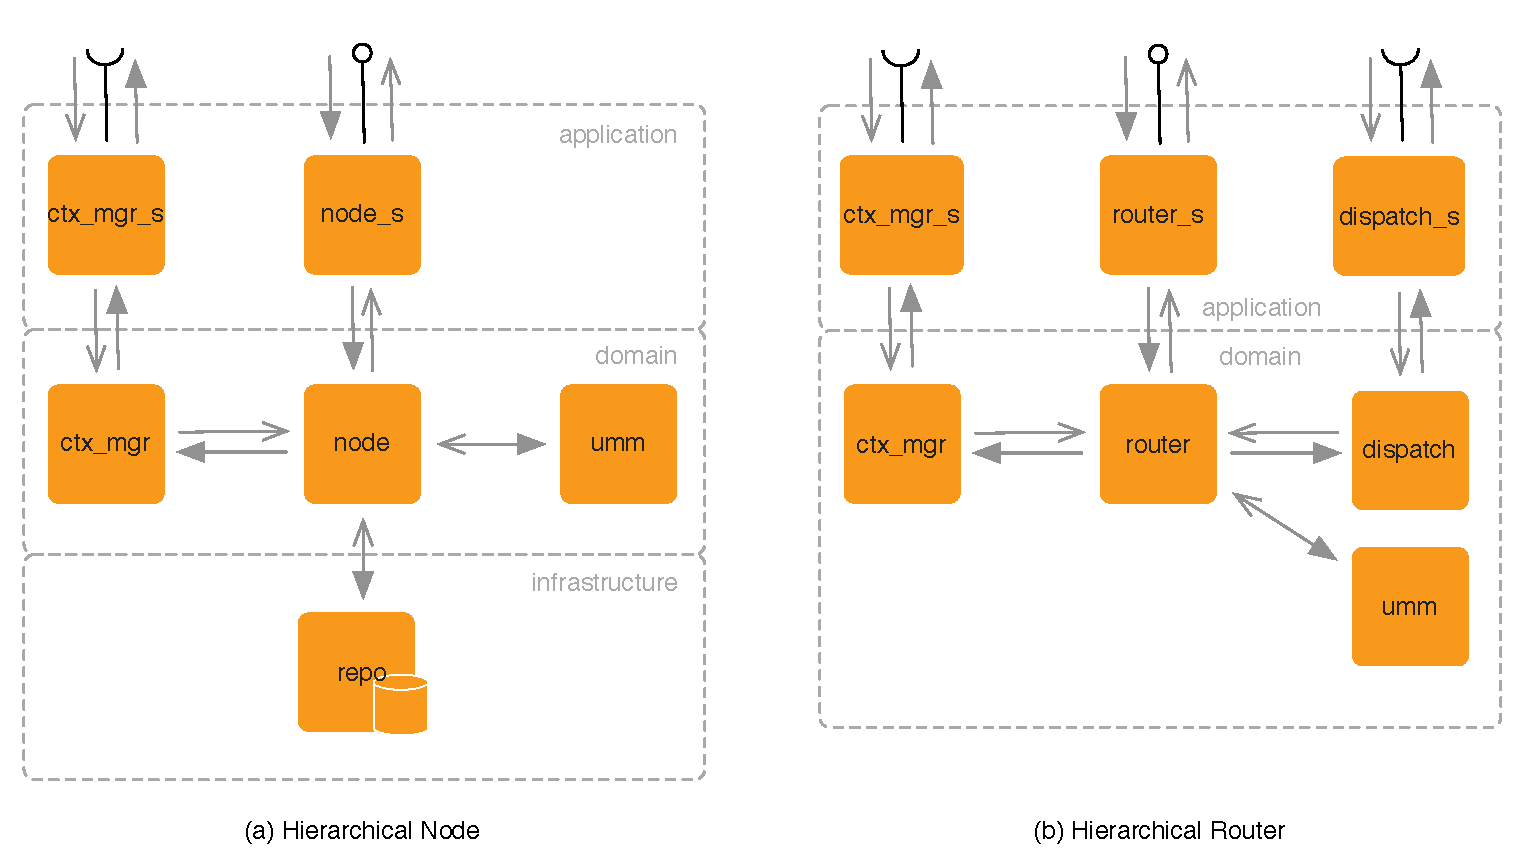
\includegraphics[width=3.5in]{router-node-view}}
Strictly layered architecture within nodes:
{\small
\begin{itemize}
\item {\bf Application} --- REST Interfaces, network access
\item {\bf Domain} --- Domain functionality, specific node/router logic and UM
\item {\bf Infrastructure} --- Data storage repositories, data objects and policies
\end{itemize}
}
\end{frame}

\section{Theoretical Foundations}
\begin{frame}
\frametitle{Distributed Security Decisions}
In order to make security decions, we must know the {\it environment} of the {\it resource} (the data object) and the {\it subject} (the user).
\pause
\newline
\newline
\newline
\begin{beamerboxesrounded}[shadow]{Fundamental Foundations}
In order to understand that our decisions are valid and maintain security in distributed {\it environments}, we must {\it prove} that local security decisions provide a compliant global solution. 
\end{beamerboxesrounded}
\pause
\newline
\newline
\newline
We make {\it greedy} with respect to security, and for efficiency we use {\it dynamic programming}.  For these to provide a globally optimal solution, we need to show that the routing problem exibits {\it optimal structure} and {\it overlapping subproblems}.
\end{frame}

\begin{frame}
\frametitle{Optimal Substructure}
{\it Idea}: If we then have a path $P$ consisting of nodes and edges $\lbrace V, E \rbrace$, that path was assembled by choosing the most secure edge $e \in E$ from a corresponding node $v \in V$ at some time $t$.  The path $P$ consisting of these edges $e$ is then the most secure path that can be chosen.
\pause
\newline
\newline
{\it Proof by Contradiction}
{\small
\begin{enumerate}
\item Assume a path $P = \lbrace V, E \rbrace$ chosen using a greedy algorithm.
\item Assume that $P$ is not the most secure, and that a more distinctly secure path $P' = \lbrace V, E' \rbrace$ exists.
\item If $P'$ exists, then at some $v \in V$ $\exists$ $e' \in E$ such that $e'$ is more secure than the corresponding edge $e \in E$.
\item If so, then at all$v \in V$, $e' = e$ leading to $E' = E$ and $P' = P$, so $P'$ is not distinct from $P$. 
\end{enumerate}
}
\pause
\color{blue}
{\small
This is essentially the shortest path problem.  In this case possible solutions are constrained however, because we don't have access to information about the entire network.  We can only evaluate context at each node.
}
\color{black}
\end{frame}

\begin{frame}
\frametitle{Overlapping Subproblems}
{\it Idea}: We can caluculate a context to determine the security posture of a given edge.  If the parameters involved in calulating that value don't change, then the security value of that edge won't change either.
\pause
\newline
\newline
{\it Proof by Contradiction}
{\small
\begin{enumerate}
\item Assume a security value $v$ associated with an edge $e \in E$ calucuated via contributing parameters $p \in P$ by an idempotent security function $f$.
\item Assume $\exists$ an alternative security value $v'$ for $e$ calculated from the same parameters $p$ by $f$.
\item Then the function $f$ returns different outputs $O$ based on the same input $p$.
\item $\not \exists$ $v'$ due to the definition of idempotence. 
\end{enumerate}
}
\color{blue}
{\small
The security functions are deterministic and don't incorporate any random behavior, so we can assume idempotence as a characteristic.
}
\color{black}
\end{frame}

\section{Implementation Overview}
\begin{frame}
\frametitle{Implementation Overview --- Environment}
The simulation environment runs over a nation-spanning overlay network hosted via Rackspace Cloud and Amazon Elastic Compute Cloud (EC2).  The network uses ICN concepts in interface design and operational semantics.
\pause
\newline
\newline
\centering
Overlay Technical Components
\begin{table}[tp] %
\centering %
\begin{tabular}{lc}
\toprule %
$Category$ 				& $Components$ 								\\\toprule %
$Infrastructure$ 		& Amazon S3, Amazon EC2, Rackspace Servers 	\\\midrule
$Operating Systems$		& Ubuntu 11.04, Ubuntu 12.04 				\\\midrule
$Technologies$			& Ruby (Sinatra, Capistrano, YAML) 			\\\midrule
$Supporting Systems$	& Git, Github 								\\\bottomrule
\end{tabular}
\caption{Supporting Components}
\end{table}
\end{frame}

\begin{frame}
\frametitle{Implementation Overview --- Capistrano}
\end{frame}

\begin{frame}
\frametitle{Implementation Overview --- Rest API}
\end{frame}

\begin{frame}
\frametitle{Implementation Overview --- Flow}
\end{frame}

\begin{frame}
\frametitle{Implementation Overview --- Usage}
{\tiny
\begin{table}[tp] %
\centering %
\begin{tabular}{lccccc}
\toprule %
\emph{Dimension}		& \emph{Type}	& \emph{Required?}	& \emph{Domain A}	& \emph{Domain B}	& \emph{Domain C} 	\\\toprule
\emph{Affiliation} 	& Set 			& Yes 				& tropic\_thunder, 	& tropic\_thunder,	& tropic\_thunder, 	\\
					&				&					& gallant\_entry	& gallant\_entry	& curious\_response	\\\midrule
\emph{Sensitivity} 	& Ordering 		& Yes 				& unclassified,		& unclassified		& unclassified,		\\
					&				&					& secret,			& secret,			& secret,			\\
					&				&					& top\_secret		& top\_secret		& top\_secret		\\\midrule
\emph{Category}		& Set 			& No 				& aqua,				& alpha,			& one,				\\
					&				&					& magenta,			& beta,				& two,				\\
					&				&					& vermillion		& gamma				& three				\\\midrule
\emph{Organization}	& Set 			& Yes 				& Oceania, 			& Oceania,			& Oceania,			\\
					&				&					& Eastasia,			& Eastasia,			& Eastasia,			\\
					&				&					& Urasia			& Urasia			& Urasia				\\\midrule
\emph{Device}	 	& Set 			& No 				& workstation, 		& workstation,		& workstation, 		\\
					&				&					& tablet,			& phone				& tablet			\\
					&				&					& phone				& 					& 					\\\midrule
\end{tabular}
\caption{All Possible Attributes for Usage Management Decisions}
\label{table:model:network-attributes}
\end{table}
}
\end{frame}

\begin{frame}
\frametitle{Implementation Overview --- Policy}
\begin{lstlisting}[language=ruby, label=lst:policy-dsl, caption=Policy DSL Example]
foobar
\end{lstlisting}
\end{frame}

\section{Final Steps}
\begin{frame}
\frametitle{Next Steps}
\end{frame}

\end{document}

